
\chapter{評価}
\label{sec:eval}
本章では,提案手法の評価を行う.


\section{評価環境}
\label{sec:eval_env}
評価環境について説明する.性能やタグ比較回数を評価するために,SimpleScalar v.3.0a をベースに作成したシュミレータを使用した.評価で仮定したプロセッサ構成を\tab{base_config}に示す.

提案手法の各種パラメータを,\tab{subseg_config}と\tab{non_subseg_config}に示す.これらのパラメータは,5\% 程度の性能低下と引き換えにできるだけ多くのタグ比較回数削減を達成できるよう,実験によって求めた最適なパラメータである.\tab{subseg_config} はSWITCH 方式をサブ・セグメントと併用する場合に最適なパラメータを,\tab{non_subseg_config} はサブ・セグメントを使用しない場合に最適なパラメータを示している.各パラメータの評価に関しては,で説明する.

測定ベンチマークには,SPEC CPU 2017 ベンチマークのうち,int 系 9 本と fp 系 9 本の計 18 本を使用した.プログラムの入力には ref データ・セットを用いた.ベンチマークの測定区間は,プログラムの先頭から 16B 命令をスキップした後の 100M 命令である.

\begin{table}[htb]
  \caption{プロセッサの基本構成}
  \footnotesize
  \center
    \begin{tabular}{l|l} \hline \hline
     Pipeline width & 8 instructions wide for each of \\
     & fetch, decode, issue, and commit \\
     Reorder buffer & 300 entries \\
     IQ & 128 entries \\
     Load/Store queue & 128 entries \\
     Physical registers & 300(int) + 300(fp) \\
     Branch prediction & 16KB Perceptron predictor~\cite{Jimenez2001} \\
     & 2K-set 4-way BTB \\
     & 10-cycle misprediction penalty \\
     Function unit & 4 iALU, 2 iMULT, \\
     &  3 FPU, 2 LSU \\
     L1 D-cache & 32KB, 8-way, 64B line \\
      & 2-cycle hit latency \\
     L1 I-cache & 32KB, 8-way, 64B line \\
      &  2-cycle hit latency \\
     L2 cache & 2MB, 16-way, 64B line \\
      & 12-cycle hit latency \\  
     Main memory & 300-cycle latency \\
     & 8B/cycle bandwidth \\ 
     Prefetch & stream-based,32-stream tracked,  \\ 
     & 16-line distance, 2-line degree, \\
     & prefetch to L2 cache \\ \hline
  \end{tabular}
  \label{tab:base_config}
\end{table}

\begin{table}[tb]
  \caption{提案手法のパラメータ構成(サブ・セグメント使用)}
  \footnotesize
  \center
    \begin{tabular}{l|l} \hline \hline
    メイン・セグメント数 & 8 \\
    サブ・セグメント数 & 2 \\
    切り替えインターバル & 10K instructions \\
    ISR しきい値 & 15\% \\
    LLC MPKI しきい値 & 2.0 \\ \hline 
  \end{tabular}
  \label{tab:subseg_config}
  \caption{提案手法のパラメータ構成(サブ・セグメント不使用)}
  \footnotesize
  \center
    \begin{tabular}{l|l} \hline \hline
    メイン・セグメント数 & 8 \\
    サブ・セグメント数 & 2 \\
    切り替えインターバル & 10K instructions \\
    ISR しきい値 & 15\% \\
    LLC MPKI しきい値 & 2.0 \\ \hline 
  \end{tabular}
  \label{tab:non_subseg_config}
\end{table}

\subsection{ベンチマークの分類}
提案手法は,プログラムの ILP や MLP に着目した制御を行う.そこで,SPEC CPU 2017 ベンチマークを ILP が高いベンチマーク,MLP が高いベンチマーク,いずれも低いベンチマークの 3 種類に分類する.ここて,ILP が高い及びMLP が高いベンチマークとは,次の条件を満たすベンチマークである.
\begin{itemize}
  \item ILP:IPCが 3.5以上のベンチマーク
  \item MLP:LLC MPKI が2 以上のベンチマーク
\end{itemize}

分類結果を\tab{classification}に示す.また,以降に示す図において,ILP(青色) 及びMLP(赤色)の表記は,そのベンチマークが ILP もしくは MLP が高いことを表す.
\begin{table}[htb]
  \caption{ベンチマークの分類}
  \footnotesize
  \center
    \begin{tabular}{c|l} \hline \hline
    high ILP & exchange2, leela, xz, bwaves\\
             & cactuBSSN, cam4, imagick\\
             & nab, pop2, roms\\ \hline
    high MLP &  omnetpp, xalancbmk, lbm\\ \hline
    low ILP and low MLP & deepsjeng, mcf\\
                        & perlbench, x264, fotonik3d\\ \hline
  \end{tabular}
  \label{tab:classification}
\end{table}

\section{評価結果:提案手法の効果}
提案手法によるタグ比較回数の削減と性能低下に関して評価を行う.評価モデルは以下の 4 種類である.
\begin{itemize}
  \item BASE:セグメント化しない通常の IQ を使用するモデル
  \item AGGRESSIVE:提案手法において常に AGGRESSIVE モードで実行するモデル
  \item CONSERVATIVE:提案手法において常に CONSERVATIVE モードで実行するモデル
  \item SWITCH:提案手法の SWITCH 方式を使用するモデル 
\end{itemize}

なお,評価に関してはサブ・セグメントを使用しない場合と使用する場合に関してそれぞれ評価を行う.

\begin{figure}[htb]
  \centering
  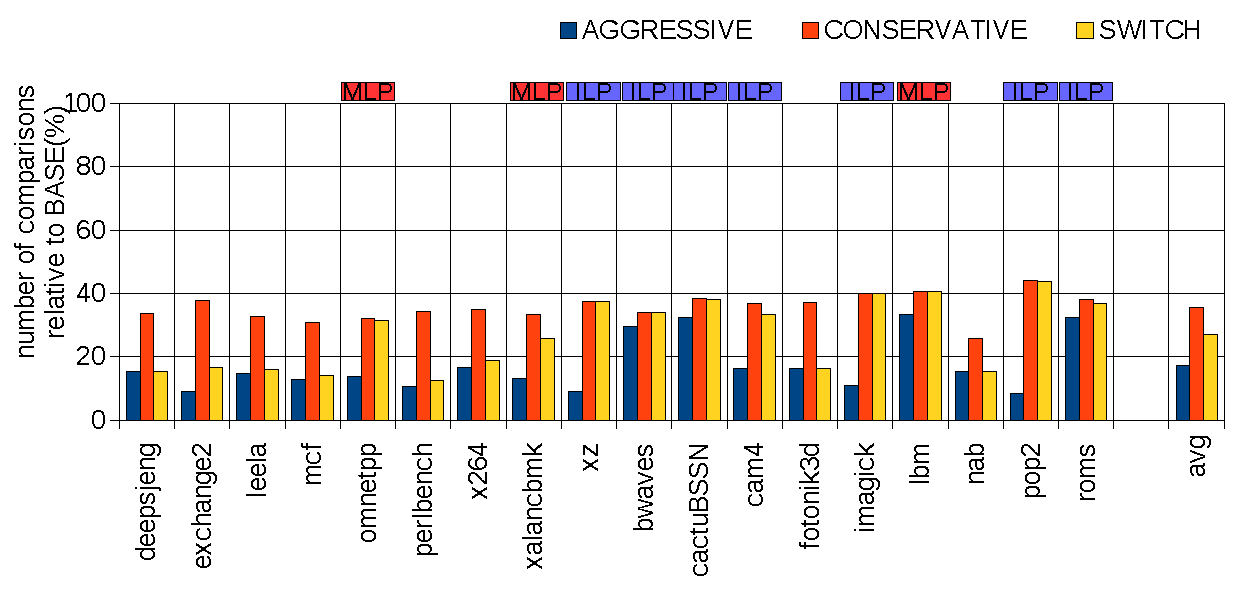
\includegraphics[keepaspectratio, scale=.8]{comp_16_1}
  \caption{提案手法によるタグ比較回数の削減(16, 1)}
  \label{fig:comp_16_1}
\end{figure}
\begin{figure}[htb]
  \centering
  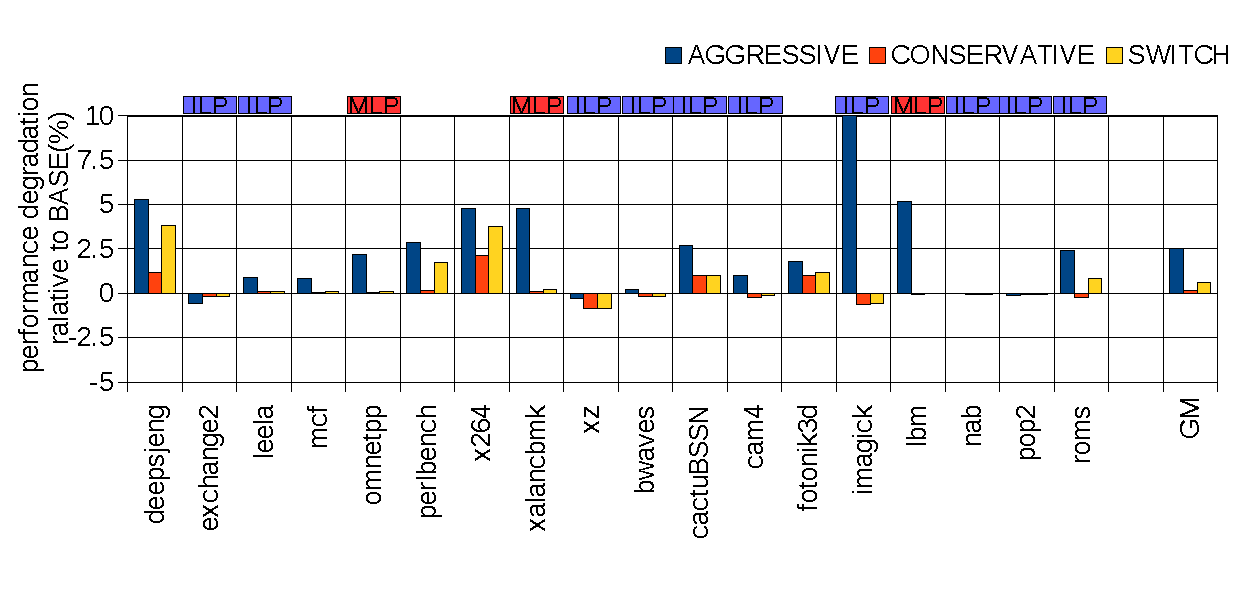
\includegraphics[keepaspectratio, scale=.8]{ipc_16_1}
  \caption{提案手法による性能低下(16,1)}
  \label{fig:ipc_16_1}
\end{figure}
\begin{figure}[htb]
  \centering
  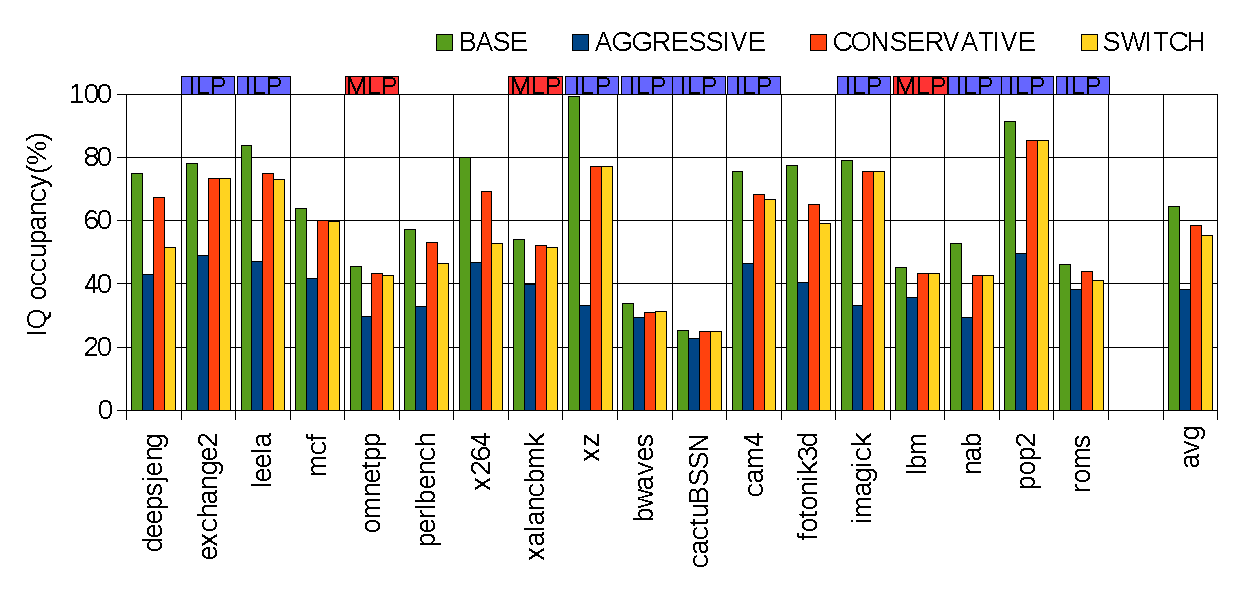
\includegraphics[keepaspectratio, scale=.8]{occupancy_16_1}
  \caption{IQ の占有率の変化(16,1)}
  \label{fig:occupancy_16_1}
\end{figure}

\subsection{サブ・セグメントを使用しない場合}
サブ・セグメントを使用しない場合の提案手法に関して評価する.提案手法に関するパラメータは\tab{non_subseg_config}に示したものを使用する.セグメント数は 16 であり,(16, 1)と表記する.

\subsubsection{タグ比較回数の削減}
\fig{comp_16_1}に,提案手法の BASE モデルに対するタグ比較回数の割合をベンチマークごとに示す.AGGRESSIVE と CONSERVATIVE のタグ比較回数削減に関しては、同図より,いずれのベンチマークにおいても,AGGRESSIVE のほうがタグ比較回数が少ないことがわかる.その差は 平均で 20\% 程度となっており,AGGRESSIVE モードのタグ比較回数を積極的に削減できるという性質が確認できる。

同図より SWITCH 方式では,平均で BASE モデルの 30\% 程度のタグ比較回数となっており,70\% の削減を達成している.

SWITCH 方式では,ILP や MLP の高いベンチマークにおいてはCONSERVATIVE と同程度のタグ比較回数であるのに対して,そうでないベンチマーク(deepsjeng,x264など)においては AGGRESSIVE に近いタグ比較回数となっていることがわかる.したがって,発行キューの容量効率が重要でないベンチマークにおいては,AGGRESSIVE モードを選択して積極的にタグ比較回数の削減が行えていることがわかる.

\subsubsection{性能低下}
\fig{ipc_16_1}に,BASE に対する提案手法による性能低下をベンチマークごとに示す.同図より,SWITCH 方式による性能低下は最大で 4\% 程度であり,多くのベンチマークでは 0\% に近く性能はほとんど低下しないということが確認できる.

SWITCH 方式の有効性に関して述べる.同図より,ILP や MLP が高い cactusBSSN や imagick,lbm などのベンチマークにおいて,AGGRESSIVE では大きく性能低下しているのに対して,CONSERVATIVE では性能低下が抑制されていることが分かる.そして SWITCH では,CONSERVATIVE と同程度の性能低下にとどまっている.従って,容量効率が性能にとって重要なプログラムにおいて,SWITCH 方式によって性能低下が抑制できていることが分かる.

\fig{occupancy_16_1}に各モデルでの発行キューの占有率を示す.占有率とは,発行キューの全エントリのうち使用された割合であり,この値が BASE のそれに近いほど容量効率が低下していないことを示す.

同図より,AGGRESSIVE では BASE に対して占有率が大きく低下しているのに対して, CONSERVATIVE では占有率の低下がある程度抑制できていることが分かる.そして,ILP や MLP が高いベンチマークでは SWITCH 方式での占有率が CONSERVATIVE と同程度となっていることが分かる.このことからも,SWITCH 方式では,容量効率の性能に対する重要性に応じて適切にモードを選択し,容量効率の低下による性能低下を抑制できており, SWITCH 方式が有効であるとわかる.

\fig{ipc_16_1}より,いくつかのベンチマークでは性能が僅かに向上していることが分かる.この理由に関して説明する.一般にランダム・キュー方式の発行キューには,命令がプログラム順に並んでいないため,最も優先して発行すべき命令の発行が遅れる可能性があるという欠点が存在する.ランダム・キューでは,命令の並びが年齢についてランダムになる一方,選択論理は,下のエントリほど優先して発行命令を選択するため,レディ命令が発行幅以上に存在する発行コンフリクトが生じた場合,誤った優先度で命令を選択することが生じる.

提案手法では発行キューの容量効率が低下するため,発行キュー内の命令数が少なくなり,結果的に発行コンフリクトが生じる確率が低下し,問題が生じにくくなり,僅かに性能が向上する.また,ILP や MLP が高いにもかかわらず,AGGRESSIVE においても性能低下の小さいベンチマークがあることが分かる.こういったベンチマークにおいても,発行コンフリクトの緩和による性能向上が発生しているため,容量効率の低下による性能低下が小さいと考えられる.

\begin{figure}[htb]
  \centering
  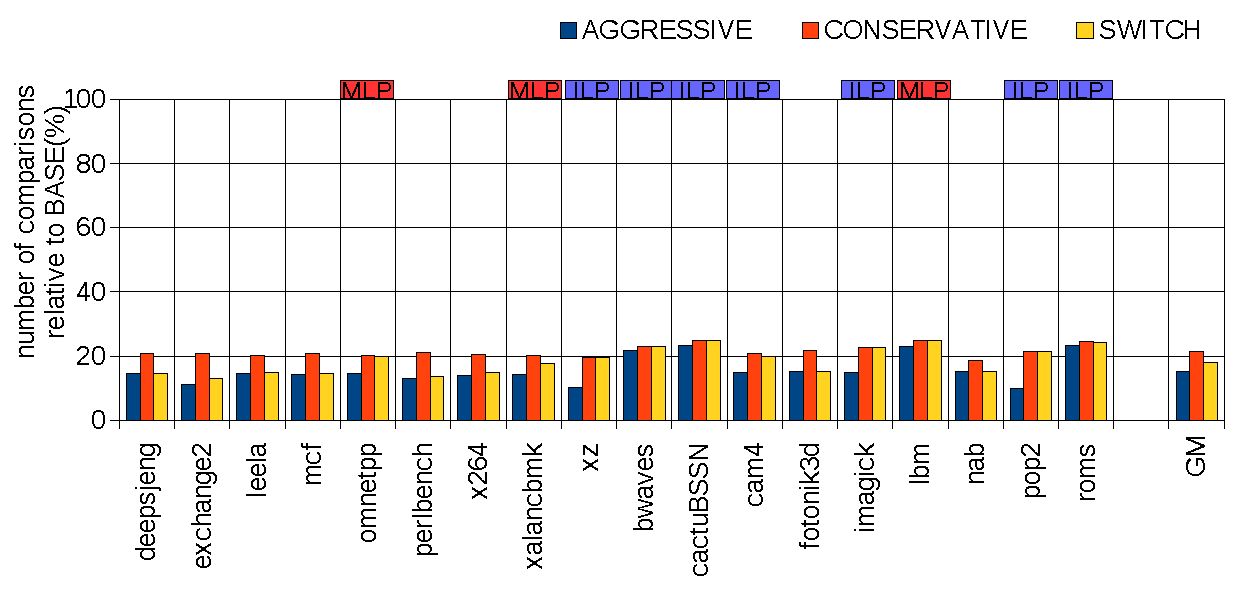
\includegraphics[keepaspectratio, scale=.8]{comp_8_2}
  \caption{提案手法によるタグ比較回数の削減(8, 2)}
  \label{fig:comp_8_2}
\end{figure}
\begin{figure}[htb]
  \centering
  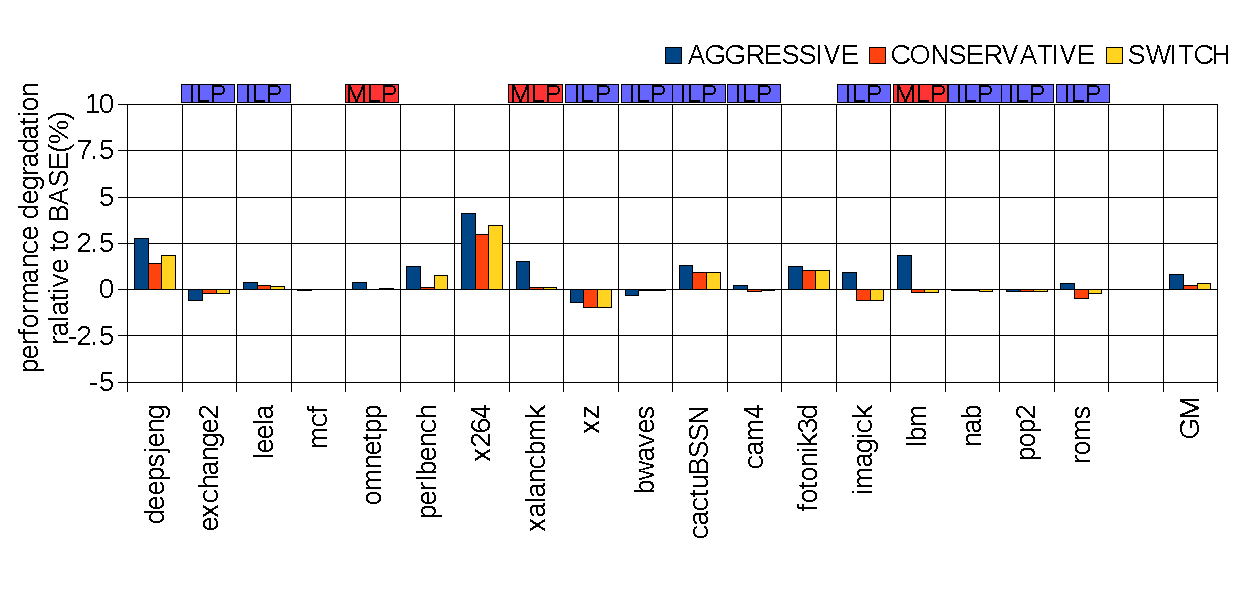
\includegraphics[keepaspectratio, scale=.8]{ipc_8_2}
  \caption{提案手法による性能低下(8,2)}
  \label{fig:ipc_8_2}
\end{figure}
\begin{figure}[htb]
  \centering
  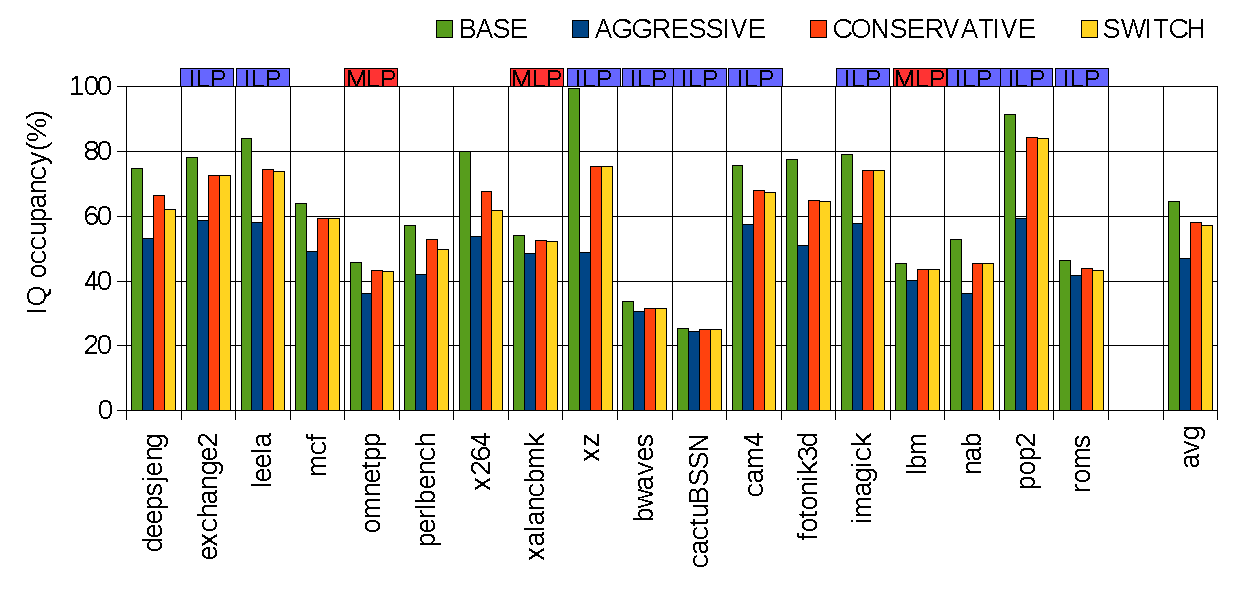
\includegraphics[keepaspectratio, scale=.8]{occupancy_8_2}
  \caption{IQ の占有率の変化(8,2)}
  \label{fig:occupancy_8_2}
\end{figure}
\begin{figure}[htb]
  \centering
  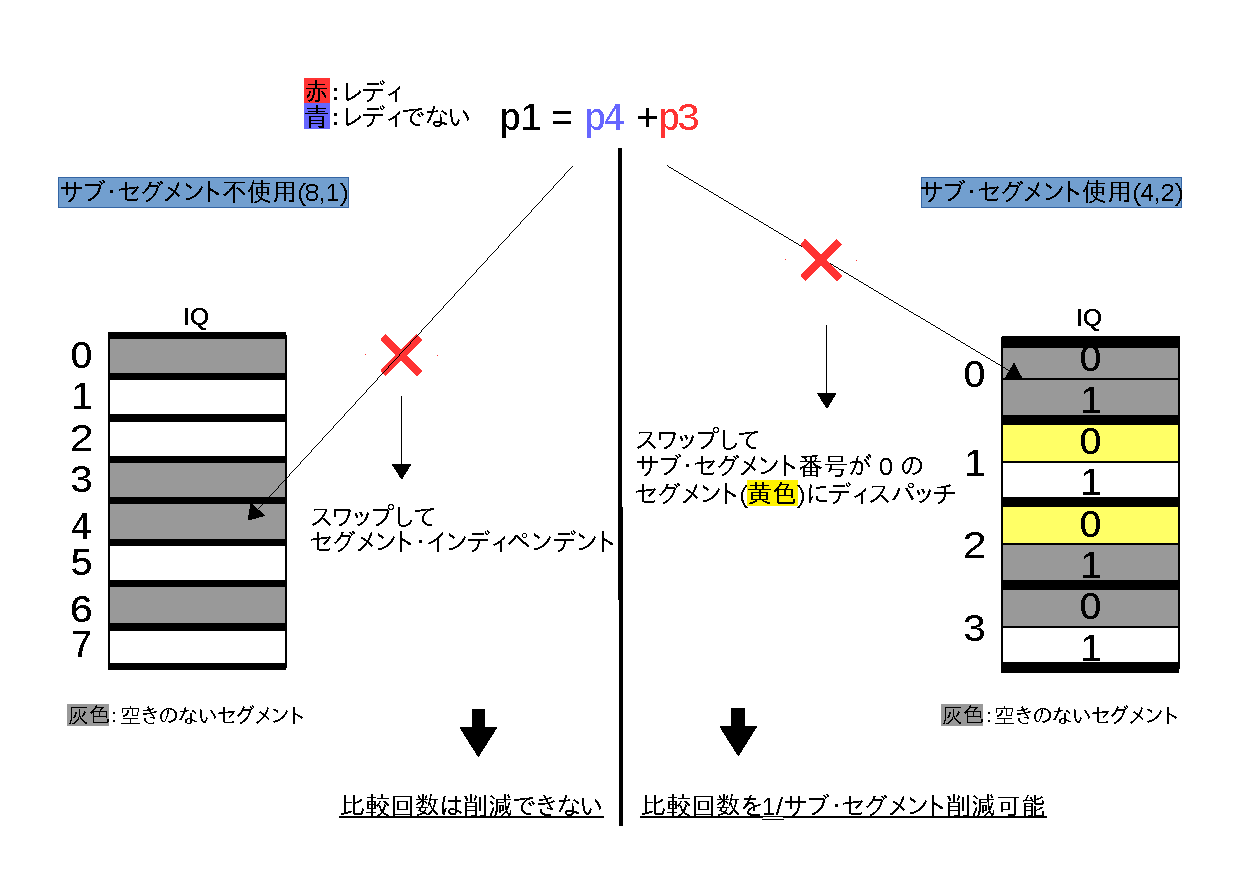
\includegraphics[keepaspectratio, scale=.8]{conservative_sub_seg}
  \caption{サブ・セグメントと CONSERVATIVE モードの組み合わせ}
  \label{fig:conservative_sub_seg}
\end{figure}

\subsection{サブ・セグメントを使用する場合}
サブ・セグメントを使用する場合の提案手法に関して評価する.提案手法に関するパラメータは\tab{subseg_config}に示したものを使用する.メイン・セグメント数は 8,サブ・セグメント数は 2 であり,(8, 2)と表記する.

\subsubsection{タグ比較回数の削減}
\fig{comp_8_2}に,提案手法の BASE モデルに対するタグ比較回数の割合をベンチマークごとに示す.AGGRESSIVE と CONSERVATIVE を比較すると,(16, 1)の場合と同様に,AGGRESSIVE のタグ比較回数が少ないことが分かる.

セグメントの総数が同じである (16, 1)と (8, 2)の CONSERVATIVE を比較すると,(16, 1)の場合が平均で 40\% 程度であるのに対して, (8, 2) では 20 \% 程度と,(8, 2)のほうがより削減できていることが分かる.これは,サブ・セグメントを使用する場合,\refsec{two_mode}で説明した CONSERVATIVE モードでのストールの回避を行った際にも,タグ比較の削減が可能となるためである.\fig{conservative_sub_seg}を用いて詳しく説明する.

図に示す命令をディスパッチする場合を考える.サブ・セグメントを使用しない場合(図左側),第 1 ソース・タグ $p4$ によって決定されるセグメント(第 4 セグメント)に空きがなければ,CONSERVATIVE ではスワップを行い,セグメント・インディペンデントとしてディスパッチを行う.この場合,第 1 ソース・タグ $p4$ のタグ比較回数は削減されない.

一方で,サブ・セグメントを使用する場合(図右側),第 1 ソース・タグ$p4$によってメインセグメントが決定され,もし空きがなければ,スワップを行う.そして,第 1 ソース・タグ $p4$ によってサブ・セグメント番号が決定され,該当する番号のいずれかに空きがあれば(図中の黄色で示したセグメント),そのセグメントディスパッチする.このとき,第 1 ソース・タグ $p4$ の比較は,タグの下位ビットがサブ・セグメント番号と一致する場合のみ行われるため,その比較回数は$1/sub\_segment\_num$ だけ削減が可能となる.

以上で説明したように,サブ・セグメントを用いると,CONSERVATIVE モードでストールの回避を行った際にも,タグ比較の削減が可能となる.その結果,\fig{ipc_8_2}で示すような CONSERVATIVE モードでの高いタグ比較削減率を達成することが出来る.

最後に SWITCH 方式に関して評価する,平均で BASE モデルの 20\% 程度のタグ比較回数となっており,80\% の削減を達成している.これは,セグメントの総数が同じである(16, 1) と比較しても高い削減率であり,サブ・セグメントが有効であると言える.

\subsubsection{性能低下}
\fig{ipc_8_2}に,BASE に対する提案手法による性能低下をベンチマークごとに示す.同図より,SWITCH 方式による性能低下は最大で 4\% 程度であり,多くのベンチマークでは 0\% に近く性能はほとんど低下しないということが確認できる.

AGGRESSIVE の性能低下率に関して考える.(8,2) では,(16,1)と比較して AGGRESSIVE の性能低下率が低いことが分かる.これは,サブ・セグメントによって AGGRESSIVE モードでの容量効率の低下が抑制されているためであると考えられる.\fig{occupancy_16_1}と\fig{occupancy_8_2}の占有率を比較すると,(16, 1)の場合は平均で 40\% 程度であった占有率が(8, 2)では,平均で 50\% となっている.また,imagick に関して見てみると,(16,1)の AGGRESSIVE では占有率が 30\% 程度で,性能低下が10\% であるのに対して, (8,2) の AGGRESSIVE では占有率が 60\% 近くまで上昇しており,その結果性能低下が 2\% 以下となっている.

以上の考察から,セグメントの総数が同じである場合,サブ・セグメントを使用することによって,AGGRESSIVE モードでの容量効率の低下による性能低下を抑制できることがわかった.

最後に,SWITCH 方式の有効性に関して説明する.(8, 2)の場合,サブ・セグメントが非常に有効である結果,AGGRESSIVE での大幅な性能低下が見られないため,(16,1)の場合と比較して SWITCH 方式の有効性は高くないように見られる.しかし, imagick や lbm などのベンチマークにおいては AGGRESSIVE で発生する性能低下を抑制できている.また,サブ・セグメントを使用しているため,CONSERVATIVE でのタグ比較削減率が高く,その結果 SWITCH 方式自体のタグ比較削減率も高くなっている.

\section{SWITCH 方式のしきい値に関する評価}
SWITCH 方式において,ILP と ILP の高低を判定するために使用するしきい値に関する評価を行う.

評価の流れとしては,まずサブ・セグメントを使用しない(16,1)の場合で評価を行う.そして,(16,1)の場合に最適とされたしきい値が,サブ・セグメントを使用する(8,2)の場合においても有効かどうかを確認する.

\begin{figure}[htb]
  \centering
  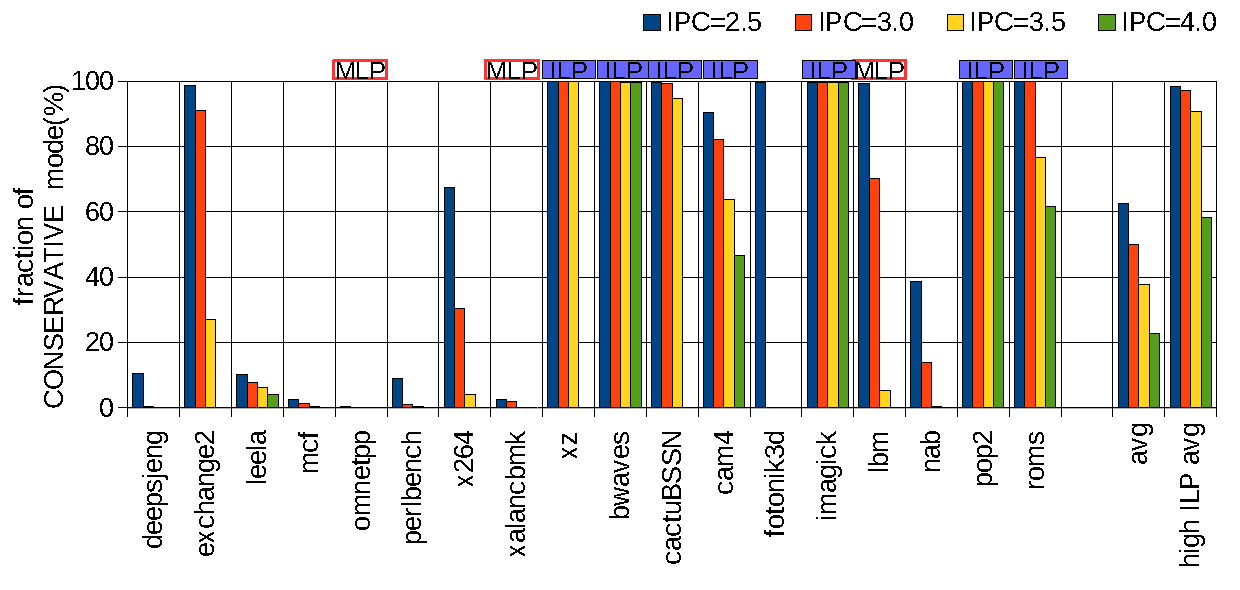
\includegraphics[keepaspectratio, scale=.8]{switch_IPC_rate}
  \caption{IPC による SWITCH 方式の制御}
  \label{fig:switch_IPC_rate}
\end{figure}
\begin{figure}[htb]
  \centering
  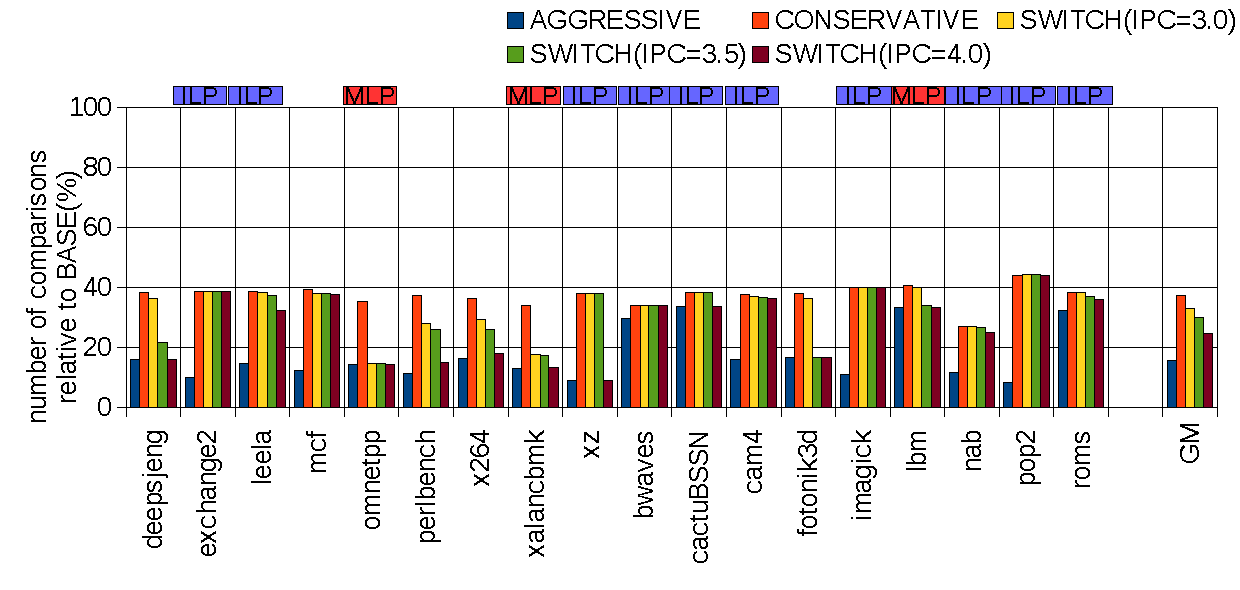
\includegraphics[keepaspectratio, scale=.8]{switch_IPC_comp}
  \caption{IPC による制御を行った SWITCH 方式によるタグ比較削減}
  \label{fig:switch_IPC_comp}
\end{figure}
\begin{figure}[htb]
  \centering
  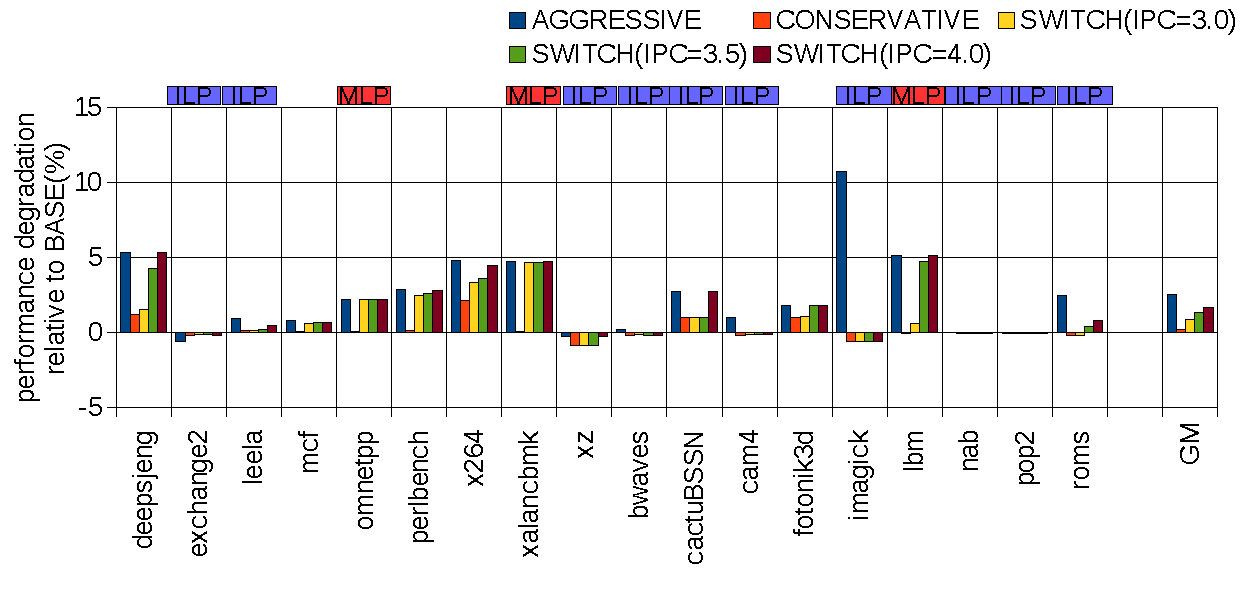
\includegraphics[keepaspectratio, scale=.8]{switch_IPC_performance}
  \caption{IPC による制御を行った SWITCH 方式による性能低下}
  \label{fig:switch_IPC_performance}
\end{figure}

\subsection{ILP の評価値:IPC}
ILP の評価として,IPC を使用する場合の評価を行った.本評価は,セグメントの数を(16,1)で行った.また,ILP による SWITCH 方式の制御のみ行い,MLP による制御は行っていない.

\subsubsection{IPC のしきい値の評価}
\fig{switch_IPC_rate}に,IPC のしきい値を変化させた場合の,AGGRESSIVE モードで実行される割合を示す.各判例の IPC=X は,ILP が高いと判定する IPC のしきい値をX とした場合を表す.また,avg は全ベンチマークの平均を,high ILP avg は ILP の高いベンチマークでの平均を示している. 

当図より,しきい値の IPC が高くなるほど,AGGRESSIVE で実行される割合が多くなっていることが分かる.これは,ILP が高いと判定される基準が厳しくなるためである.ILP の高いベンチマークに関して見ると,多くのベンチマークにおいて,しきい値が 3.5 の場合は AGGRESSIVE モードの割合が高いが,しきい値が 4.0 になると AGGRESSIVE モードの割合が急激に増加していることが分かる.high ILP avg を見ると,しきい値が 3.5 の場合は AGGRESSIVE モードの割合は 5\% 程度であるが,しきい値が 4.0 の場合は AGGRESSIVE モードの割合は 35\% 程度と高くなる.

ILP が高い場合は CONSERVATIVE モードで実行することが望ましい.従って,IPC のしきい値は,3.5 程度が適当であるといえる.

\subsubsection{しきい値の違いによる提案手法のタグ比較削減と性能低下}